% !TeX root = ../main.tex

\chapter{Second Quantization}

\section{QM of single particle}

Dirac notation will be used in this book: ket $\ket|\Phi>$, bra $\bra<\Phi|$, and operator $\hat O$. Wave function should be $\braket<x|\Phi>$.

For single particle QM, we have six axioms (postulates)

With hamiltonian $\hat H$
\begin{enumerate}
  \item Description of a state $\ket|\Phi> \in \mathcal H$:
  \begin{itemize}
    \item Using Vector Space
    \item List
    \item Orthogonality
    \item Completeness
  \end{itemize}
  \item Observables: $\hat A \in \mathcal H$, $\hat A^\dagger = \hat A$.
  \item \item Measurements: Spectral Decomposion
  \begin{itemize}
    \item $a_n$, eigenvalue of $\hat A$.
    \item $P_n = |\braket<a_n|\Phi>|^2$
  \end{itemize}
  \item Post-measurement: collapse: $\ket|\Phi>_\text{pre} \xlongrightarrow{\text{measurement}} \ket |a_n>$
  \item $\iu\hbar\partial_t\ket|\Psi> = \mathcal H\ket|\Psi>$
\end{enumerate}

Canonical(?) Quantization rules $x \to \hat x$, $p \to \hat p$, and $[\hat x, \hat p] = \iu\hbar$,

Then you can define Poisson bracket $\{\bar x, p\} = \mathbbm I \Rightarrow [\hat x, \hat p] = \mathbbm I$.

\section{Canonical Quantisation}

\subsection{}

$\ket|x>$, $[\hat x, \hat p] = \iu\hbar$. $\hat p = -\iu\hbar \partial_x$, $\braket<x|\Phi>$.

$\braket<\hat p|\Phi>$, $\hat p \to p$, $\hat x \to \iu\hbar\partial p$.

For classical string like

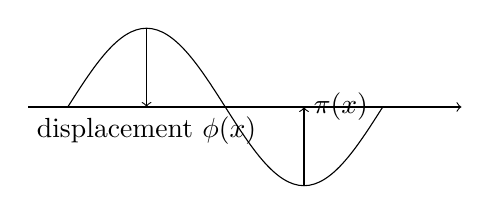
\begin{tikzpicture}
  \draw [->] (-.5,0) -- (5,0);
  \draw (0,0) sin (1,1) cos (2,0) sin (3,-1) cos (4,0);
  \draw [->] (1,1) --++ (0,-1) node [below] {displacement $\phi(x)$};
  \draw [->] (3,-1) --++ (0,1) node [right] {$\pi(x)$};
\end{tikzpicture}
\begin{equation}
  \mathcal H  = \int \d x\ab(\frac T2(\nabla_x\phi(x))^2
              + \frac1{2\rho}\pi^2(x)\ab)
  \footnote{Physically, it should have more terms}
\end{equation}
Exactly, $\iu\{\tilde\phi,\tilde\pi\} = 1$.

Quantisation $[\hat\phi(x),\hat\pi(y)] = \iu\hbar\delta(x - y)$.

\subsection{Harmonic oscillator: zero-dim field theory}

The hamiltonian, eigen energy and state are
\begin{equation}
  H = \frac{p^2}{2m} + \frac12 m\omega^2x^2,~
  E_n = \ab(n + \frac12)\hbar\omega,~
  \ket|n> = \frac{1}{\sqrt{n!}}(a^\dagger)^n\ket|0>
\end{equation}
Let
\[
  \xi = \frac x{\Delta x},~               p_\xi = \frac p{\Delta p},~
  \Delta x = \sqrt{\frac\hbar{m\omega}},~ \Delta p = \sqrt{m\omega\hbar}
\]
then we have
\begin{equation}
  \begin{cases}
    a^\dagger = \frac1{\sqrt2}(\xi - \iu p_\xi)\\
    a         = \frac1{\sqrt2}(\xi + \iu p_\xi)
  \end{cases} \qq{and}
  \begin{cases}
    [a,a^\dagger] = 1\\
    [a,a] = [a^\dagger,a^\dagger] = 0
  \end{cases}
\end{equation}
Do it differently, the time evolution
\begin{equation}
  x(t) = \braket<\phi_n(t)|\hat x|\phi_n(t)>
  = \braket<\phi_n|\upe^{iHt/\hbar} \hat x\upe^{-iHt/\hbar}|\phi_n>
  = \braket<\phi_n|\hat x(t)|\phi_n>
\end{equation}
and the EOM (Equation of Motion) is
\begin{equation}
  -\iu\hbar\odv{a(t)}t = [H,a(t)] = \omega a(t)
\end{equation}
So,
\begin{equation}
  \hat x(t) = \frac{\Delta x}{\sqrt2}[a(t) + a^\dagger(t)],~
  \hat p(t) = \frac{\Delta p}{\iu\sqrt2}[a(t) - a^\dagger(t)]
\end{equation}
These type of operators are so called \emph{field operators}.

\begin{equation}
  \int_{-\Delta}^{+\Delta}\d xe^{-x^2-gx^4} \text{Herry Ponc$\hat o$}
= \lim_{N \to \infty} \lim_{\Delta \to \infty}
\end{equation}
\begin{enumerate}
  \item $j, (\pi_j)^2 + (D_j - D_{j+1})^2$: chiral phonon, theormal hall.
\end{enumerate}

\section{QM of many particles}

Seventh Axiom:
If you don't consider anything: we want to remove exchange degeneracy
$\Rightarrow$ symmetrization / antisymmetrization rule.

Two types wavefunctions. For Boson: permanent; for Fermison slater dert.

Each state is one particle in
particle lable $\varphi_1^{\epsilon_1}$, $\varphi_2^{\epsilon_2}$, $\ldots\,$,~$\varphi_m^{\epsilon_m}$, which $\epsilon_i \approx \epsilon_j$, and state lable $1$, $2$, $\ldots\,$,~$N$.
\[
  \begin{pNiceMatrix}[first-row, first-col]
      & \varphi_1^{\epsilon_1} & \varphi_2^{\epsilon_2} & \ldots & \varphi_m^{\epsilon_m}\\
    1 & \ket|1,\varphi_1^{\epsilon_1}> & \ket|1,\varphi_1^{\epsilon_2}>\\
    2 & \ket|2,\varphi_1^{\epsilon_1}>\\
    \vdots\\
    N
  \end{pNiceMatrix}
\]
symmetrical polynomials.

% Issue of continue limit:

We can get into a newer occupation number representation

label any state $\ket|\varphi> = \ket|n_{\epsilon_1}\text{(occupation / energy No.)}, n_{\epsilon_2}, \ldots, n_{\epsilon_n}, \ldots>_\text{boson / fermion}$

occupation number representation: dependent on underlying first quantization basis.
\begin{equation}
  N = n_{\epsilon_1} + \cdots + n_{\epsilon_n} + \cdots
\end{equation}

\section{Fock space}

\begin{equation}
  F = \{\mathcal H_0, \mathcal H_1, \mathcal H_2, \ldots, \mathcal H_n, \cdots\}
\end{equation}

Rock matrix:
\begin{equation}
  \begin{pNiceMatrix}[first-row,]
    \ket|\varphi, N = 0> & \ket|\varphi, N = 1>\\
    H_0\\
        & H_1\\
        &     & \ddots\\
        &     &         & H_N\\
        &     &         &     & \ddots
  \end{pNiceMatrix}
\end{equation}

\section{Field operators}

Suppose we have
\begin{equation}
  \ket|\Psi> = \ket|\qquad>;~
\end{equation}
$\Psi(x)$: $\braket<x|\Psi>$.

Each state has a particular wave function,

$\ket|x_1>$ is given by $\Psi^\dagger(x_1)\ket|0> \Rightarrow \hat x\ket|0> = \hat a + \hat a^\dagger\ket|0> = \ket|1>$.

We are creating $a^\dagger\ket|0>$, $\ket|x>\braket<x|1> = \ket|x_1>\psi_1(x_1)$.

Project $a^\dagger$ onto $\ketbra|x><x|$, that is
\[\psi^\dagger(x) = a^\dagger\ketbra|x><x|\]
Similarly, if u want two particles at two different positions, u get
\begin{equation}
  \psi^\dagger(x_2)\psi^\dagger(x_1)\ket|0> = \ket|x_1,x_2> = \psi^\dagger(x_2)\ket|x_1>
\end{equation}
They are commutation
\begin{equation}
  \psi^\dagger(x)\psi^\dagger(y) = \pm\psi^\dagger(y)\psi^\dagger(x)
  \Leftrightarrow [\psi^\dagger(x), \psi^\dagger(y)]_\mp\footnote{$[A,B]_\mp = AB \mp BA$} = 0
\end{equation}

And finally, introduce
\[[\hat\psi(x),\hat\psi(y)] = 0, \hat\psi(x)\ket|0> = 0\]
For any state like $\ket|\Psi> \in F$, u also see like $\braket<\Psi|\psi(x)|\psi> = \braket<\Psi|\psi^\dagger(x)|\psi> = 0$.

$\braket<\varphi, N|\varphi, N - 1> = 0$.
And finally, we want to be able to
$\braket<y|x> = \delta(x - y) = \braket<y|\psi^\dagger(x)|0> = \braket<0|\hat\psi(y)|x>$.
u can prove that:
$\hat\psi(x)\ket|y> = \delta(x - y)$, and finally
$[\hat\psi(x),\hat\psi(y)]_\mp = \delta(x - y)$.

\section{Creation / annilation operators}

For any state $\braket<x|n> = \varphi_n(x)$, and u can also $\ket|n> = \int \d x$.

\begin{framed}
  IDENTITY IS VERY IMPORTANT! $\mathbbm 1$
  \[\mathbbm 1 = \int \d x\ketbra|x><x|\]
\end{framed}
Then we have
\[
  \ket|n> = \int\d x\ket|x>\braket<x|n> = \int\d x\varphi_n(x)\ket|x> = \int\d x\varphi_n(x)\psi^\dagger(x)\ket|0>
\]
u can define $\Rightarrow d_n^\dagger = \int\d x \varphi_n(x)\psi^\dagger(x) \Rightarrow d_n^\dagger\ket|0> = \ket|n>$.

Similarly, $\Rightarrow \hat d_n \equiv \int \d x\varphi_n^*(x)\tilde\psi(x)$: $\Rightarrow \hat d_n\ket|n> = \ket|0>$. So $\hat d_n\ket|n> \to \hat d_n\hat d_n^\dagger\ket|0>$ (Homework)

Also prove that $[d_n, d_m^\dagger]_\pm = \braket<n|m> = \delta_{n,m}$

In other words, ...

% 20250909
\section*{Occupation  number rep.}

for $\ket|x_1, ..., x_n>$,
if u change any particle like (reverse $x_1$ and $x_n$), u will get
$(t)^p\ket|x_1,x_2,...,x_n>$. $(t)^p$: boson \& fermion.

interchange: $1 ~ 2 ~ 3 \to 2 ~ 1 ~ 3$ (Permutation) $\#P$ ($P_{1\to2}$, $P_{2\to1}$): $\#$ of perm speration needed.

 When take $\mod_2(p)$,

 $h_o:\ \epsilon_1, \epsilon_2, \ldots, \epsilon_i \to \ket|n_1, n_2, \ldots, n_i,...>_{b(P)} \Rightarrow$ Fock space: $H_0 \oplus H_1 \oplus ... H_N \oplus ...$

Creation and annilation operators: $d_{n_i}^\dagger$, $d_{n_i}$
$\Leftrightarrow \psi^\dagger(x)\ket|0> = \ket|x>$

$d_n^\dagger \ket|0> = \ket|n>$, $d_n^\dagger = \frac1{\sqrt{n!}}(a^\dagger)^n$

Identity
\[\mathbbm 1 = \frac1{N!}\sum_{n_1, ..., n_i} \ketbra|n_1,n_2,n_3,...><...| = \int \d x\ketbra|x><x| = \int \d x\psi^\dagger(x)\cancel{\ketbra|0><0|}\psi(x) = \int \d x_1 \ldots \d x_n \ketbra|x_1,...,x_i><...|\]

\section{Hamiltonians in second quantization}

Operators of total number of particles
\begin{equation}
  \hat N = \int \d x\hat n(\bm x), ~ \hat N(\bm x) = \psi^\dagger(\bm x)\psi(\bm x),~ \hat N = \sum_n d_n^\dagger d_n, \hat N_n = d_n^\dagger d_n
\end{equation}

$\hat n(\bm x) \ket|n_1\ldots ...> \to \sum \ket|x_1,...,x_i,...>$

Eignevalue is equal to $(\sum_i\delta(x - x_i))\ket|x_1,\ldots, x_i, \ldots,x_N>$

$\hat h_0$: $\hat h_0\ket|\epsilon_1> = \epsilon_i\ket|\epsilon_i>$

If we have $N$ particles, for each of the particle, we have to specify a Hamiltonian
\[
  H_0 = \sum_{i=1}^N \hat h_0(\bm x)i
\]
In some occupation states, we have specify the occupation numbers
\[\ket|n_1,\ldots,n_j,\ldots>,~ \qq{while} \sum n_j = N\]
and
\[H_0\ket|n_1,\ldots,n_j,\ldots> = \sum_j\epsilon_j n_j\ket|...>\]
$\oplus$ in book $\sum \epsilon_j \ket|...>$.

Then we can define $H_0\ket|n...> = (\epsilon_{n_1} + \epsilon_{nN})\ket|...>$

\[
  H_0 = \int \d x \d x' \psi^\dagger(x)\braket<x|\hat h_0|x>\hat\psi(x')
\]
If $\hat h_0 = \hat p^2/2m$, then $\braket<x|\hat h_0|x'> = \delta(x - x_0)(-\frac{\nabla^2k^2}{2m})$
Then,
\begin{align}
  H_0 & = \sum_n \int \d x\d x'\psi^\dagger(x)\underset{\varphi_n(x')}{\braket<x|\hat h|n>}\underset{\varphi_n^*(x')}{\braket<n|x>}\hat\psi(x')\\
  & = \sum_n \int \d x\d x'\epsilon_n \varphi_n(x)\psi^\dagger(x); \varphi_n^*(x')\hat\psi(x')\\
  & = \sum_n \epsilon_n d_n^\dagger d_n = \sum_n \epsilon_n \hat N_n
\end{align}

\[[\hat N_n, d_m^\dagger]_- = \delta_{nm}d_m^\dagger, ~ [\hat N_n, d_m]_- = -\delta_{nm} d_n\]
% For SO(3) group: $[L_i, L_j] = \epsilon_{ijk}\hat L_k$, and SO(3,1) $\d s^2 = c^2\d t^2 - \d x^2 - \d y^2 - \d z^2 = \d x^2 + \d y^2 + \d z^2 - c^2\d t^2$.
Consider $[H_0, \hat d_m^\dagger] = \epsilon_m d_m^\dagger$, $[H_0,d_m] = -\epsilon_n d_m$, the we get spectral geneeratiy algtron $[H_0,\hat O]\propto \hat O$ while $H_o = \sum \epsilon_0 \ketbra|n><n|$ and $\ketbra|m><m|$

Finally, we can write
\[
  H_0 = \int \d r\psi^\dagger(r) h_{r_0}(r,\nabla_r, \sim)\psi(r)
\]
Here, $h = \braket<r|\hat h_0|r>$.

\subsection{Interactivy Hamiltonian}

Consider two body $\nu(\hat x_1, \hat x_2)$
\[
  H_\text{int}\ket|x_1,...,x_N..> = \frac12\ab(\sum_{i\neq j}\nu(\hat x_i,\hat x_j))\ket|x_1,...,x_N..>
  = \ab(\sum_{i>j}\nu(\hat x_i,\hat x_j))\ket|x_1,...,x_N..>
\]
\[\hat|x_1,...,x_n> ~ \hat n(x)\]
We write $v(\hat x_i,\hat x_j) = \int \d x' \d x\delta(x - x_i)\delta(x' - x_j) v(x,x')$ and substitute it into $H_\text{int}$, then using $(\sum_i \delta(x - x_i))\ket|x_1,...,x_i ..., x_N>$ inversely, then we have
\begin{align}
  H_\text{int} & = \frac12 \int \d x \d x'\ab(\nu(x,x')n(x)n(x') - \nu(x,x)n(x))\\
  & = \frac12 \int \d x \d x' \nu(x,x)\ab(\psi^\dagger(x)\psi(x)\psi^\dagger(x')\psi(x') - \delta(x - x')\psi^\dagger(x)\psi(x))\\
  & = \frac12 \int \d x\d x' \nu(x,x')\psi^\dagger(x)\psi^\dagger(x')\psi(x)\psi(x')
\end{align}

\subsection{Total Hamiltonian}

Such as
\begin{align*}
  \mathcal H & = \int \d x \d x' \psi^\dagger(x)\braket<x|h_0|x'>\psi'(x')
              +\frac12\int \d x \d x' \nu(x,x')\psi^\dagger(x)\psi^\dagger(x')\psi(x)\psi(x')\\
             & = \sum_{ij}h_{ij}d_i^\dagger d_j + \frac12\sum_{ijmn}\nu_{ijmn}d_i^\dagger d_j^\dagger d_m d_n
\end{align*}
Here
\[h_{ij} = \braket<i|\hat h|j> = \int \d r \varphi_i^* h_i(r,\nabla_r,\sim)\varphi_j(r) = h^*_{ji}, ~ \braket<x|i> = \varphi_i(x)\] 
and
\[
  \nu_{ijmn} = \int \d x\d x' \varphi_i^*(x)\varphi_j^*(x') \nu(x,x') \varphi_m(x')\varphi_n(x)
\]